\documentclass{standalone}

\usepackage{tikz}
\usetikzlibrary{fit}

\begin{document}
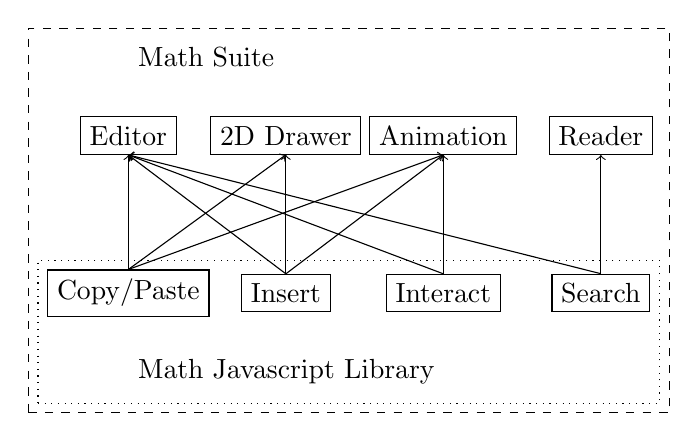
\begin{tikzpicture}
  \node[draw,rectangle] (Copy) at (0,0) {Copy/Paste};
  \node[draw,rectangle] (Insert) at (2,0) {Insert};
  \node[draw,rectangle] (Interact) at (4,0) {Interact};
  \node[draw,rectangle] (Search) at (6,0) {Search};

  \node[right] (LibraryName) at (0,-1) {Math Javascript Library};
  \node[draw,dotted,fit=(Copy) (Insert) (Insert) (Search) (LibraryName)]
  (Library){};

  \node[draw,rectangle] (Editor) at (0,2) {Editor};
  \draw[->] (Copy.north) -- (Editor.south);
  \draw[->] (Insert.north) -- (Editor.south);
  \draw[->] (Interact.north) -- (Editor.south);
  \draw[->] (Search.north) -- (Editor.south);
  \node[draw,rectangle] (2D) at (2,2) {2D Drawer};
  \draw[->] (Copy.north) -- (2D.south);
  \draw[->] (Insert.north) -- (2D.south);
  \node[draw,rectangle] (Animation) at (4,2) {Animation};
  \draw[->] (Copy.north) -- (Animation.south);
  \draw[->] (Insert.north) -- (Animation.south);
  \draw[->] (Interact.north) -- (Animation.south);
  \node[draw,rectangle] (Reader) at (6,2) {Reader};
  \draw[->] (Search.north) -- (Reader.south);

  \node[right] (SuiteName) at (0,3) {Math Suite};
  \node[draw,dashed,fit=(Library) (SuiteName)] {};
\end{tikzpicture} \\
\end{document}
